\begin{appendices}

%
% The first appendix must be "Self-appraisal".
%
\chapter{Self-appraisal}

% <This appendix should contain everything covered by the 'self-appraisal' criterion in the mark scheme. Although there is no length limit for this section, 2---4 pages will normally be sufficient. The format of this section is not prescribed, but you may like to organise your discussion into the following sections and subsections.>

\section{Critical self-evaluation}

Broadly speaking I would say the project was a success, although there were certainly things I would do differently if I were to do it again. The quality of the notebooks are quite high, and I feel the content I decided to cover was covered well. This being said, there is also room for a lot more and I wish I had managed my time better in order to be able to cover these topics. One of the main reasons I chose this area of research was due to my interest in fluid flow problems and the Naiver-Stokes equations. In order to learn about these, I had to first obtain a strong base knowledge in the finite element method, which is a fairly dense and sometimes inaccessible topic. As such, it took a long time to get to a place where I was comfortable with the majority of the terms and ideas which meant I didn't have enough time to research the fluid flow problems I chose the topic for.

The first text I read was {\em The Mathematical Theory of Finite Element Methods} by Brenner and Scott. This is a high-level mathematical text, suited for mathematicians with knowledge of functional analysis, which I lacked. This text put me off due to its complexity and made me feel that the topic was too complex for an undergraduate final year project. It gave me good initial insight however, and after finding the Bengzon-Larson textbook, I felt much more confident in the way forward, but much time had passed until I got to this point.

Another thing I would do differently is try to get more testers. Having three testers definitely impacted my ability to evaluate the success of the project effectively. The small sample size meant that individual biases stood out much more than they should have. Also none of the testers had a background in FEM, meaning potential inaccuracies in my explanations couldn't be identified as well. Cross-referencing against my sources, and taking great care was my attempt to minimise the inaccuracies, but there will undoubtedly be some present.

However, despite the drawbacks of the evaluation and problems with time management, I am personally very proud of the project. A lot of research was performed in a field I hadn't even heard of before starting. Sifting through complicated texts and tutorials developed my skills in critical reading and research.

It was interesting writing a project with a minimal amount of programming. Most projects develop a software product, and while this is still a software product, the majority of the implementation was just natural English text. This meant that past projects, while still very helpful, had many fundamental differences to mine. I think this project blurs the lines between a maths research dissertation and a computer science project, which made me doubt the validity of the idea. There were times where I thought about scrapping the idea and simply building a variety of solvers in FEniCSx, but so much time had been put into research it probably wasn't a good idea.

Also, if I had more time I would have produced a document containing the solutions to all exercises. Due to time constraints, I felt it was more important to get the content produced and out to testers instead of focusing on the ``quality of life'' aspects. If this were a real product, the solutions would be of great importance, but since I was producing a minimum viable product, they were left as an additional consideration that I unfortunately never got round to completing. It should still be noted that I did complete all exercises to ensure they had the right degree of challenge and were, in fact, soundly constructed.

\section{Personal reflection and lessons learned}

One of the main lessons learned was in time-keeping and maintaining a consistent workflow. Unfortunately, the Gantt chart proposed in Section \ref{section:development-methodology} was not stuck to and the idea of Agile development had to be scrapped. This probably effected the quality of the final product slightly and it meant that one of the initial goals of the project had to be changed. I failed to stick to the timeline I proposed for a few reasons, one of which being an unfortunate set of circumstances at home, outside of my control. However, I should still take some personal responsibility in the matter and I know I could have devoted more time at the beginning.

The problem was, I chose my modules for this academic year by choosing three quarters of my modules to be in the first semester and the other quarter in my second semester. This meant, over the course of the first term, almost no work was done towards completing the project aside from a minimal amount of reading. If I were to do this again, I would try to maintain a much more consistent workflow. I also feel I could have used the knowledge and advice of my supervisor better. Being independent is a useful skill, but knowing when to ask for help and letting others know if you are struggling is infinitely more so.

\section{Legal, social, ethical and professional issues}

\subsection{Legal issues}

For all sources used, I had to check if licensing permitted my use, replication, and modification of it. All the software sources used were open source and fell under various public licenses. All softwares that specify credit should be given have been.

\subsection{Social issues}

The only social issue that might relate to the project is the idea of education and open-source content. Education is a right that is often taken for granted, and people in developing countries may not always have access to the same resources that we do. As such, if this were a real product being released, I would make it open-source and free for everyone. With many of the proprietary and advanced FEM softwares and books on the subject being kept behind paywalls, open source tools like FEniCSx and the tutorials surrounding it are crucial to allowing people to learn all around the world. Whether they go to university or not, education should be accessible and free for all (in my opinion).

\subsection{Ethical issues}

The ethical issues of the project mainly surrounded user testing. In order to get the testers assistance, I created some user testing questionnaires explaining the project, some background information, their role within it and how their data would be stored. I specified they retain the right to leave the project at any time and that we could discuss options if they were unable to complete certain tasks. Luckily, this did not occur. They can be seen in Appendix \ref{appendix:additional-pdfs}. While they are not legally binding in any sense, they do provide a good-will basis of communication. They serve more as a consent for use of their data than a binding agreement to participate.

Outside of the consent forms, all communication regarding the project happened over Microsoft Teams and email, where I announced when notebooks were available for testing and provided links to the repository and questionnaire. Inside the repository there was a friendly but professional readme file that explained the goals of the project and what was expected of the testers.

I believe the project was conducted in an ethical and responsible way.

\subsection{Professional issues}

There were no professional issues regarding this project. No external businesses or corporations were contacted all testing happened with University Of Leeds students.

%
% Any other appendices you wish to use should come after "Self-appraisal". You can have as many appendices as you like.
%
\chapter{External Material}
%<This appendix should provide a brief record of materials used in the solution that are not the student's own work. Such materials might be pieces of codes made available from a research group/company or from the internet, datasets prepared by external users or any preliminary materials/drafts/notes provided by a supervisor. It should be clear what was used as ready-made components and what was developed as part of the project. This appendix should be included even if no external materials were used, in which case a statement to that effect is all that is required.>

This code is from J.S. Dokken's FEniCSx Tutorial \cite{fenics-tutorial} and was adapted to fit the examples presented.

\begin{lstlisting}[language=Python, caption={Solving the Poisson Equation}]
from mpi4py import MPI
from dolfinx import mesh
domain = mesh.create_unit_square(MPI.COMM_WORLD, 8, 8,
                                 mesh.CellType.quadrilateral)
from dolfinx.fem import FunctionSpace
V = FunctionSpace(domain, ("CG", 1))
from dolfinx import fem
uD = fem.Function(V)
uD.interpolate(lambda x: 1 + x[0]**2 + 2 * x[1]**2)
import numpy
# Create facet to cell connectivity required to determine boundary facets
tdim = domain.topology.dim
fdim = tdim - 1
domain.topology.create_connectivity(fdim, tdim)
boundary_facets = mesh.exterior_facet_indices(domain.topology)
boundary_dofs = fem.locate_dofs_topological(V, fdim, boundary_facets)
bc = fem.dirichletbc(uD, boundary_dofs)
import ufl
u = ufl.TrialFunction(V)
v = ufl.TestFunction(V)
from petsc4py.PETSc import ScalarType
f = fem.Constant(domain, ScalarType(-6))
a = ufl.dot(ufl.grad(u), ufl.grad(v)) * ufl.dx
L = f * v * ufl.dx
problem = fem.petsc.LinearProblem(a, L, bcs=[bc], 
          petsc_options={"ksp_type": "preonly", "pc_type": "lu"})
uh = problem.solve()
import pyvista
from dolfinx import plot
pyvista.start_xvfb()
topology, cell_types, geometry = plot.create_vtk_mesh(domain, tdim)
grid = pyvista.UnstructuredGrid(topology, cell_types, geometry)
plotter = pyvista.Plotter()
plotter.add_mesh(grid, show_edges=True)
plotter.view_xy()
if not pyvista.OFF_SCREEN:
    plotter.show()
else:
    figure = plotter.screenshot("fundamentals_mesh.png")
u_topology, u_cell_types, u_geometry = plot.create_vtk_mesh(V)
u_grid = pyvista.UnstructuredGrid(u_topology, u_cell_types, u_geometry)
u_grid.point_data["u"] = uh.x.array.real
u_grid.set_active_scalars("u")
u_plotter = pyvista.Plotter()
u_plotter.add_mesh(u_grid, show_edges=True)
u_plotter.view_xy()
if not pyvista.OFF_SCREEN:
    u_plotter.show()
warped = u_grid.warp_by_scalar()
plotter2 = pyvista.Plotter()
plotter2.add_mesh(warped, show_edges=True, show_scalar_bar=True)
if not pyvista.OFF_SCREEN:
    plotter2.show()
\end{lstlisting}

\begin{lstlisting}[language=Python, caption={Extract from Deflection of a Membrane}]
from dolfinx import geometry
bb_tree = geometry.BoundingBoxTree(domain, domain.topology.dim)
cells = []
points_on_proc = []
# Find cells whose bounding-box collide with the the points
cell_candidates = geometry.compute_collisions(bb_tree, points.T)
# Choose one of the cells that contains the point
colliding_cells = geometry.compute_colliding_cells(domain, cell_candidates, 
                                                   points.T)
for i, point in enumerate(points.T):
    if len(colliding_cells.links(i))>0:
        points_on_proc.append(point)
        cells.append(colliding_cells.links(i)[0])
points_on_proc = np.array(points_on_proc, dtype=np.float64)
u_values = uh.eval(points_on_proc, cells)
p_values = pressure.eval(points_on_proc, cells)
import matplotlib.pyplot as plt
fig = plt.figure()
plt.plot(points_on_proc[:,1], 50*u_values, "k", linewidth=2, 
         label="Deflection ($\\times 50$)")
plt.plot(points_on_proc[:, 1], p_values, "b--", linewidth = 2, 
         label="Load")
plt.grid(True)
plt.xlabel("y")
plt.legend()
# If run in parallel as a python file, we save a plot per processor
plt.savefig(f"membrane_rank{MPI.COMM_WORLD.rank:d}.png")
\end{lstlisting}
%
% Other appendices can be added here following the same pattern as above.
%

\begin{lstlisting}[language=Python, caption={The Heat Equation - Diffusion of a Gaussian Function}]
import numpy as np
from mpi4py import MPI
from petsc4py import PETSc
from dolfinx import fem, mesh, io, plot
# Define temporal parameters
t = 0 # Start time
T = 1.0 # Final time
num_steps = 50     
dt = T / num_steps # time step size
# Define mesh
nx, ny = 50, 50
domain = mesh.create_rectangle(MPI.COMM_WORLD, [np.array([-2, -2]),
              np.array([2, 2])], [nx, ny], mesh.CellType.triangle)
V = fem.FunctionSpace(domain, ("CG", 1))
# Create initial condition
def initial_condition(x, a=5):
    return np.exp(-a*(x[0]**2+x[1]**2))
u_n = fem.Function(V)
u_n.name = "u_n"
u_n.interpolate(initial_condition)
# Create boundary condition
fdim = domain.topology.dim - 1
boundary_facets = mesh.locate_entities_boundary( domain, fdim, 
                  lambda x: np.full(x.shape[1], True, dtype=bool))
bc = fem.dirichletbc(PETSc.ScalarType(0), 
                     fem.locate_dofs_topological(V, fdim, boundary_facets),
                     V)
xdmf = io.XDMFFile(domain.comm, "diffusion.xdmf", "w")
xdmf.write_mesh(domain)
# Define solution variable, and interpolate initial solution for 
# visualization in Paraview
uh = fem.Function(V)
uh.name = "uh"
uh.interpolate(initial_condition)
xdmf.write_function(uh, t)
import ufl
u, v = ufl.TrialFunction(V), ufl.TestFunction(V)
f = fem.Constant(domain, PETSc.ScalarType(0))
a = u * v * ufl.dx + dt*ufl.dot(ufl.grad(u), ufl.grad(v)) * ufl.dx 
L = (u_n + dt * f) * v * ufl.dx
bilinear_form = fem.form(a)
linear_form = fem.form(L)
A = fem.petsc.assemble_matrix(bilinear_form, bcs=[bc])
A.assemble()
b = fem.petsc.create_vector(linear_form)
solver = PETSc.KSP().create(domain.comm)
solver.setOperators(A)
solver.setType(PETSc.KSP.Type.PREONLY)
solver.getPC().setType(PETSc.PC.Type.LU)
import pyvista
pyvista.start_xvfb()
import matplotlib.pyplot as plt

grid = pyvista.UnstructuredGrid(*plot.create_vtk_mesh(V))

plotter = pyvista.Plotter()
plotter.open_gif("u_time.gif")

grid.point_data["uh"] = uh.x.array
warped = grid.warp_by_scalar("uh", factor=1)

viridis = plt.cm.get_cmap("viridis", 25)
sargs = dict(title_font_size=25, label_font_size=20, fmt="%.2e", color="black",
             position_x=0.1, position_y=0.8, width=0.8, height=0.1)

renderer = plotter.add_mesh(warped, show_edges=True, lighting=False,
                            cmap=viridis, scalar_bar_args=sargs,
                            clim=[0, max(uh.x.array)])
for i in range(num_steps):
    t += dt

    # Update the right hand side reusing the initial vector
    with b.localForm() as loc_b:
        loc_b.set(0)
    fem.petsc.assemble_vector(b, linear_form)
    
    # Apply Dirichlet boundary condition to the vector
    fem.petsc.apply_lifting(b, [bilinear_form], [[bc]])
    b.ghostUpdate(addv=PETSc.InsertMode.ADD_VALUES, 
                  mode=PETSc.ScatterMode.REVERSE)
    fem.petsc.set_bc(b, [bc])

    # Solve linear problem
    solver.solve(b, uh.vector)
    uh.x.scatter_forward()

    # Update solution at previous time step (u_n)
    u_n.x.array[:] = uh.x.array

    # Write solution to file
    xdmf.write_function(uh, t)
    # Update plot
    warped = grid.warp_by_scalar("uh", factor=1)
    plotter.update_coordinates(warped.points.copy(), render=False)
    plotter.update_scalars(uh.x.array, render=False)
    plotter.write_frame()
plotter.close()
xdmf.close()
\end{lstlisting}

\chapter{Additional Documents}
\label{appendix:additional-pdfs}

The following pages contain some additional PDFs created by me that might be of interest to the reader. All of these can also be found in the main code repository \texttt{Finite-Element-Method-Project}. The notebooks themselves have not been included here and can be found by accessing the repository.

\begin{figure}[H]
\centering
\begin{tabular}{cc}

\includegraphics[width=65mm]{images/questionnaire/preamble} & 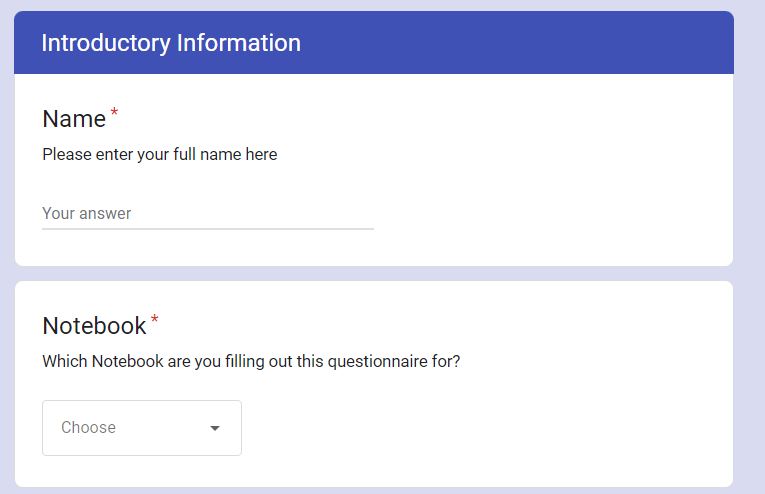
\includegraphics[width=65mm]{images/questionnaire/q0} \\
Preamble & Admin Questions \\[6pt]
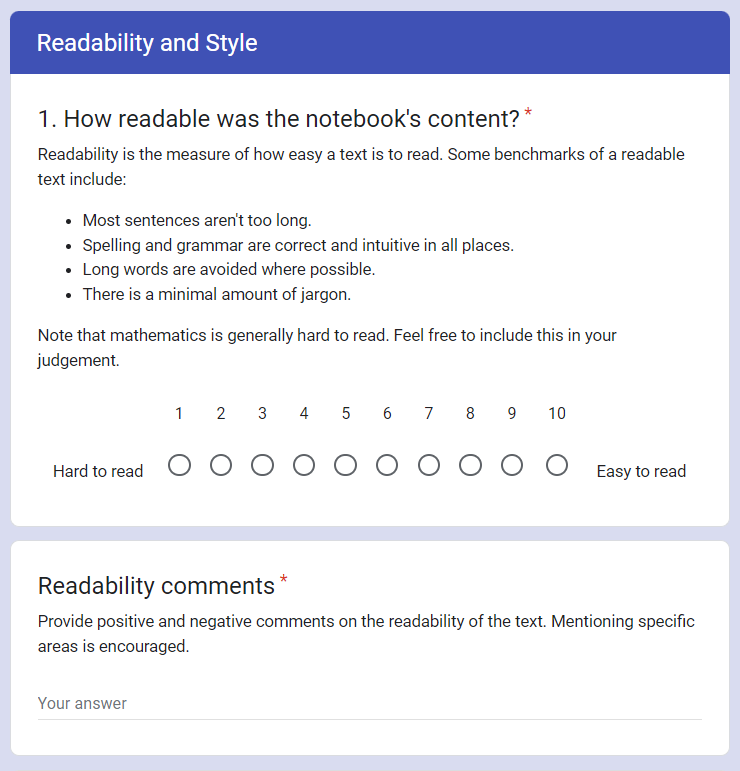
\includegraphics[width=65mm]{images/questionnaire/q1} &   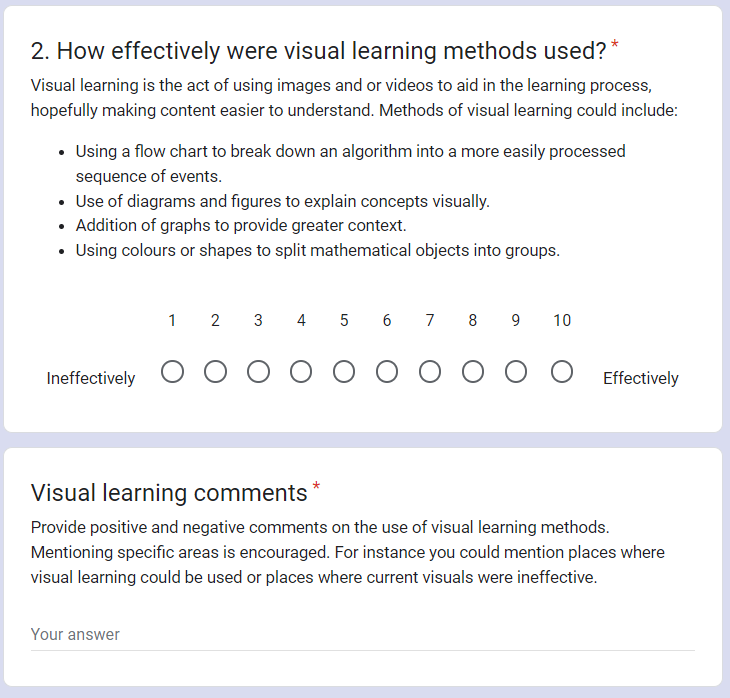
\includegraphics[width=65mm]{images/questionnaire/q2} \\
1. Readability & 2. Visual Learning \\[6pt]
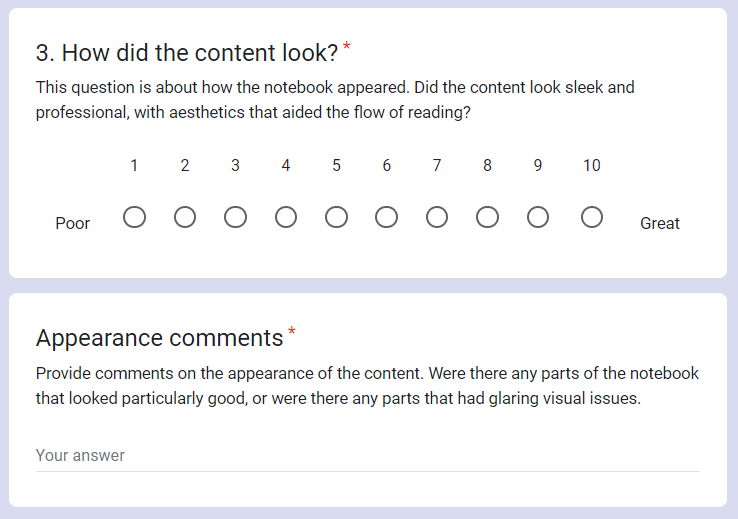
\includegraphics[width=65mm]{images/questionnaire/q3} &   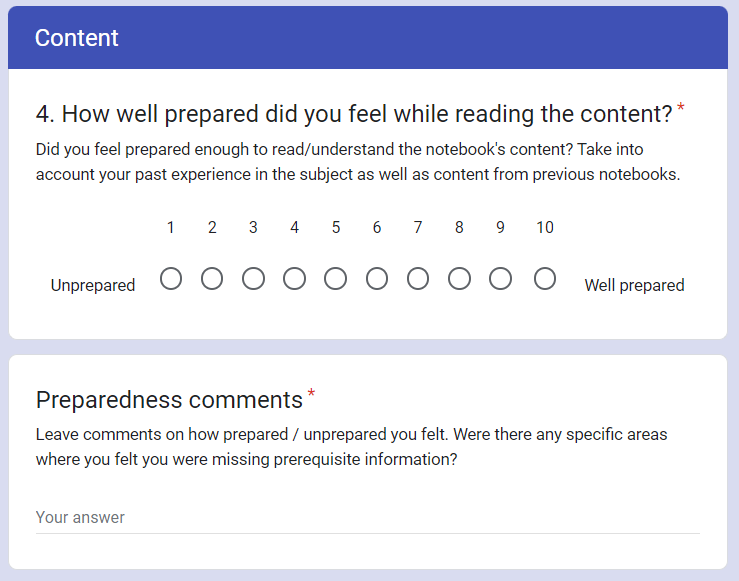
\includegraphics[width=65mm]{images/questionnaire/q4} \\
3. Aesthetics & 4. Preparedness (Pace) \\[6pt]
\end{tabular}
\end{figure}

\begin{figure}[H]
\centering
\begin{tabular}{cc}
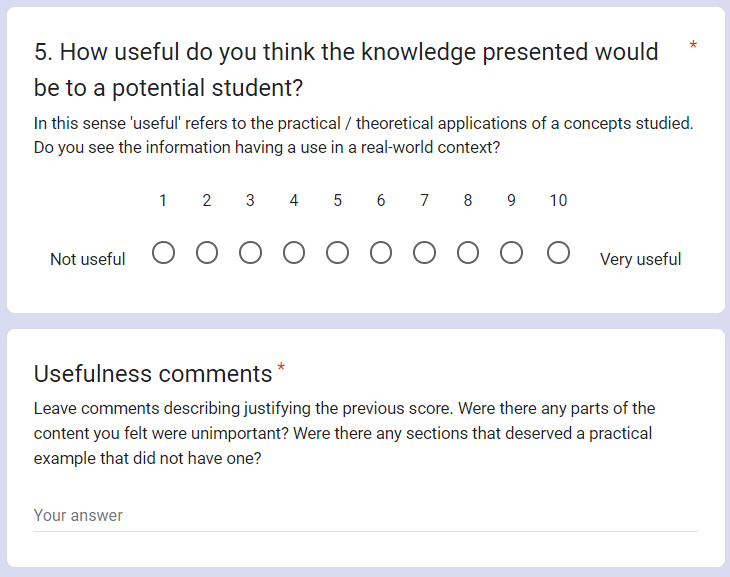
\includegraphics[width=76mm]{images/questionnaire/q5} &   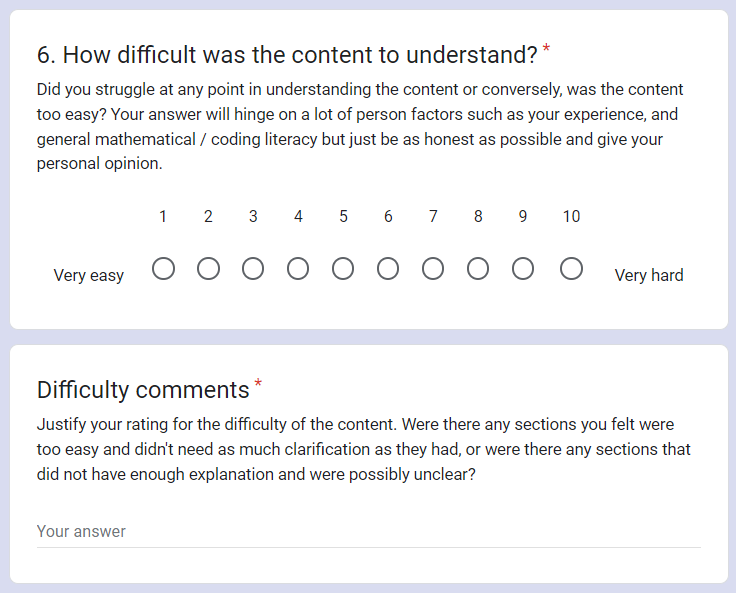
\includegraphics[width=76mm]{images/questionnaire/q6} \\
5. Usefulness & 6. Difficulty \\[6pt]
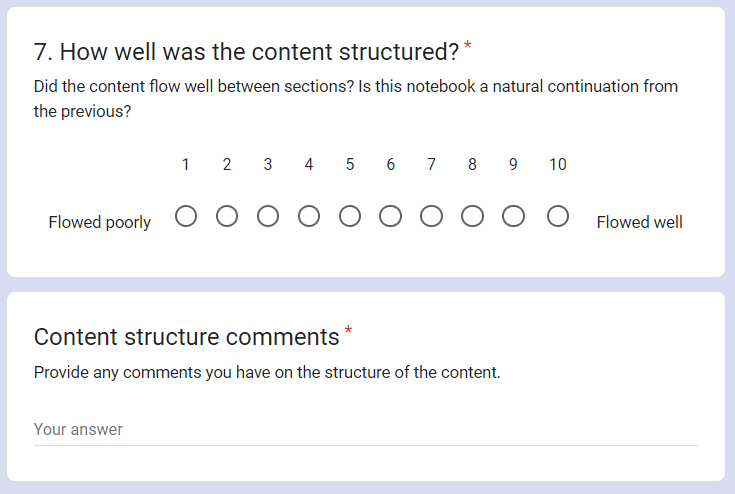
\includegraphics[width=76mm]{images/questionnaire/q7} &   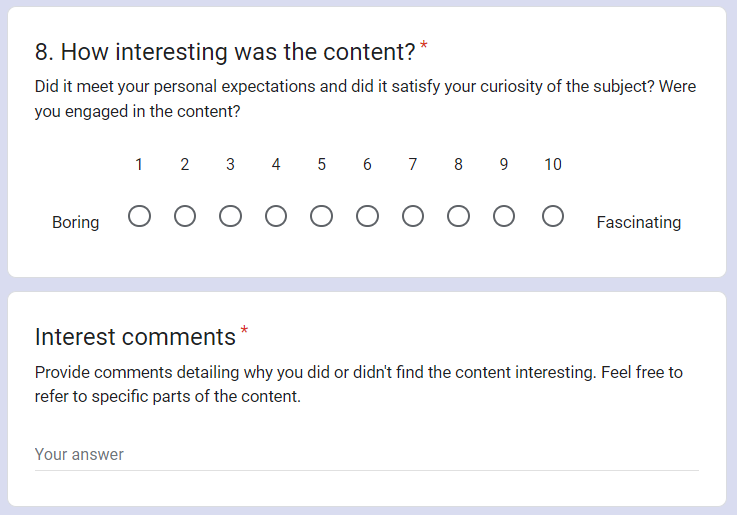
\includegraphics[width=76mm]{images/questionnaire/q8} \\
7. Structure & 8. Interest \\[6pt]
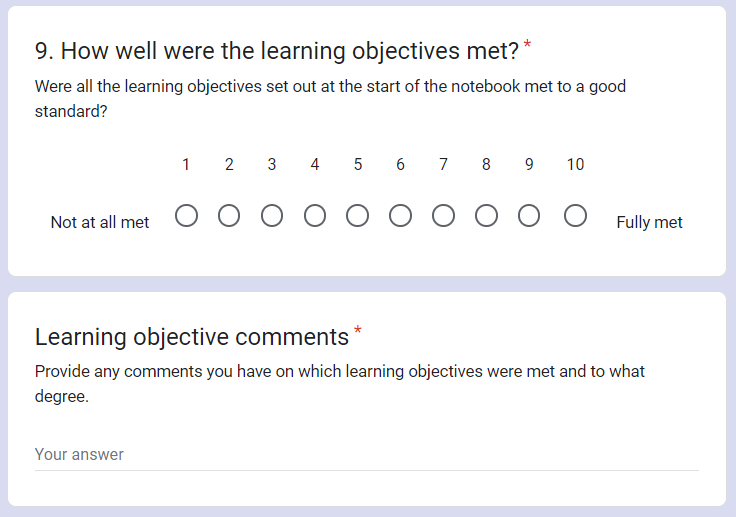
\includegraphics[width=76mm]{images/questionnaire/q9} &   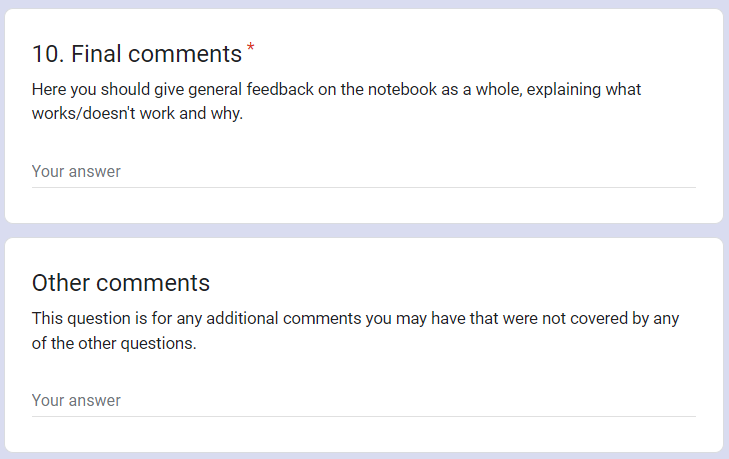
\includegraphics[width=76mm]{images/questionnaire/q10} \\
9. Learning objectives & 10. Final/Other Comments \\[6pt]
\end{tabular}
\end{figure}

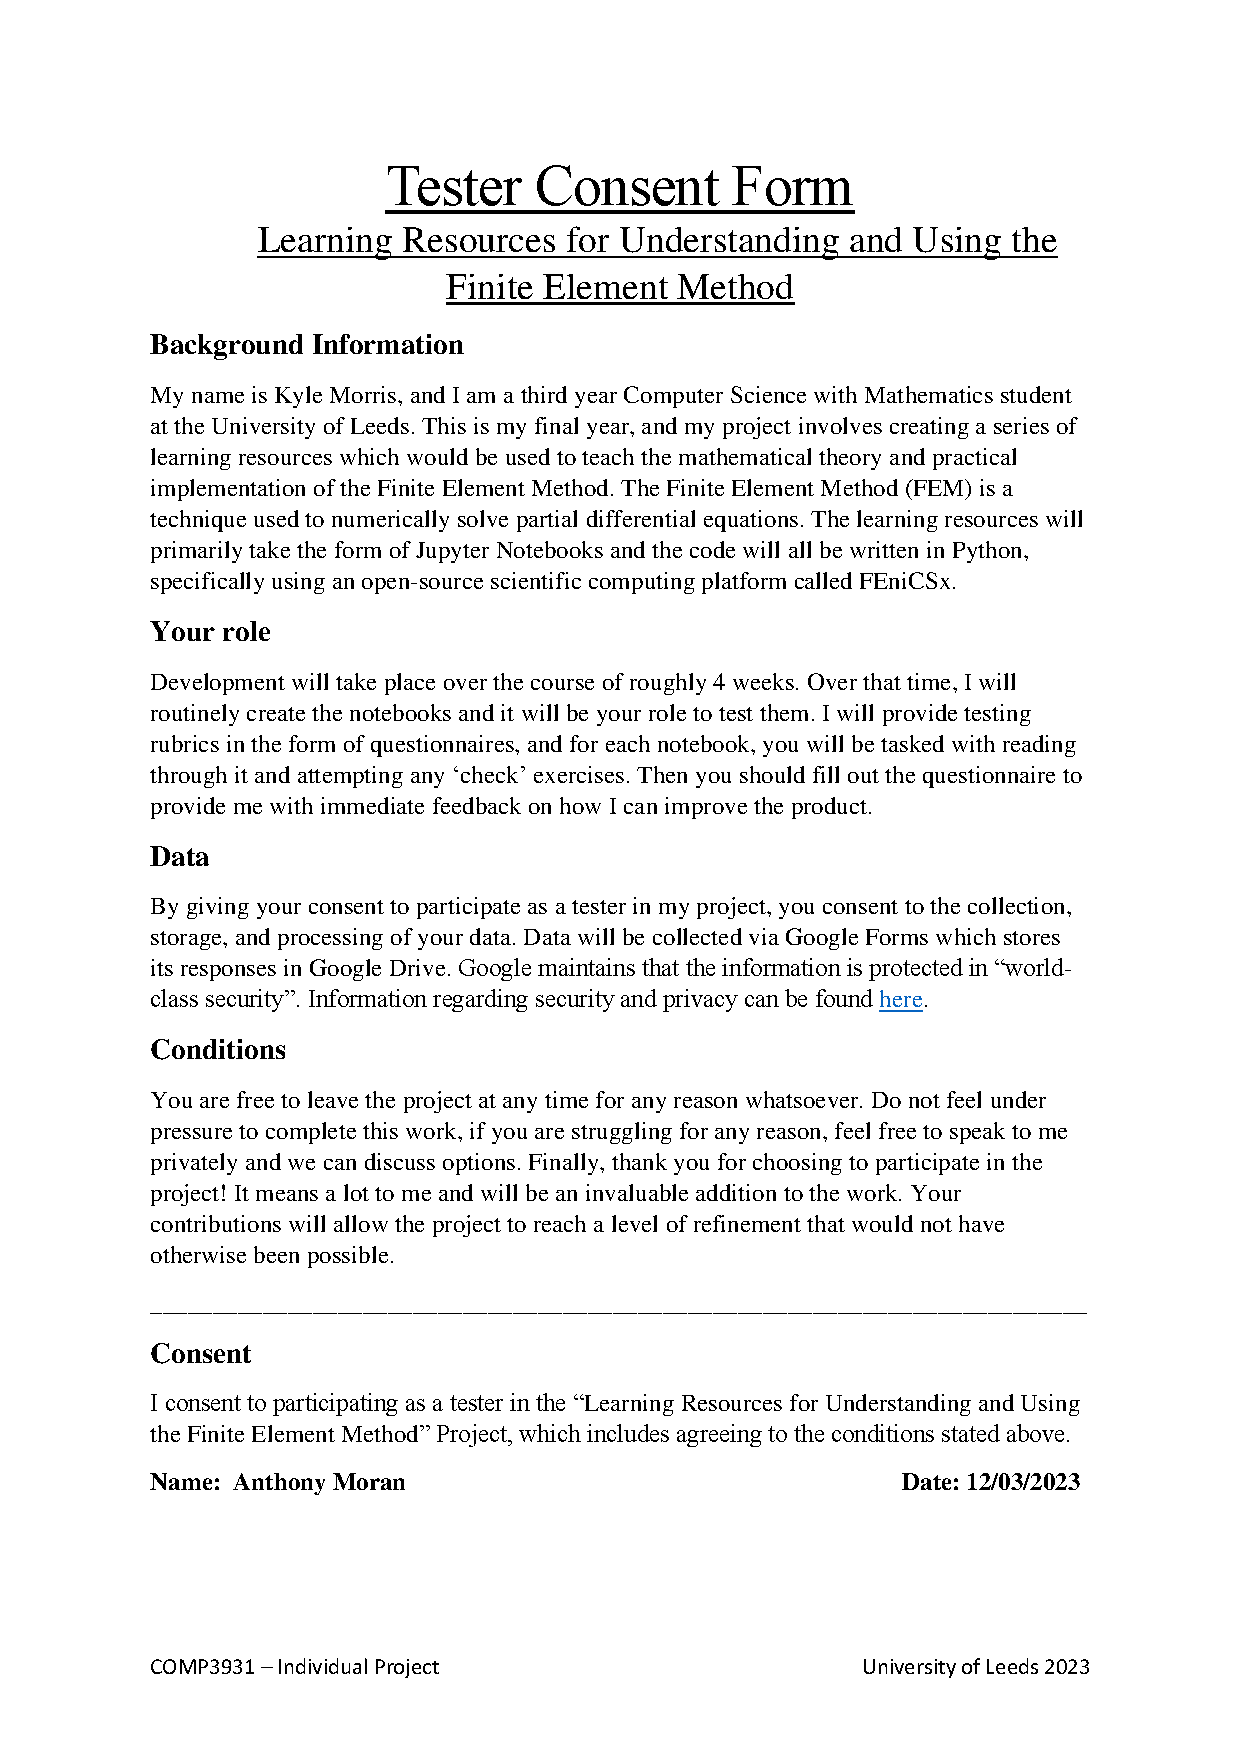
\includepdf{images/consent-forms/anthony.pdf}
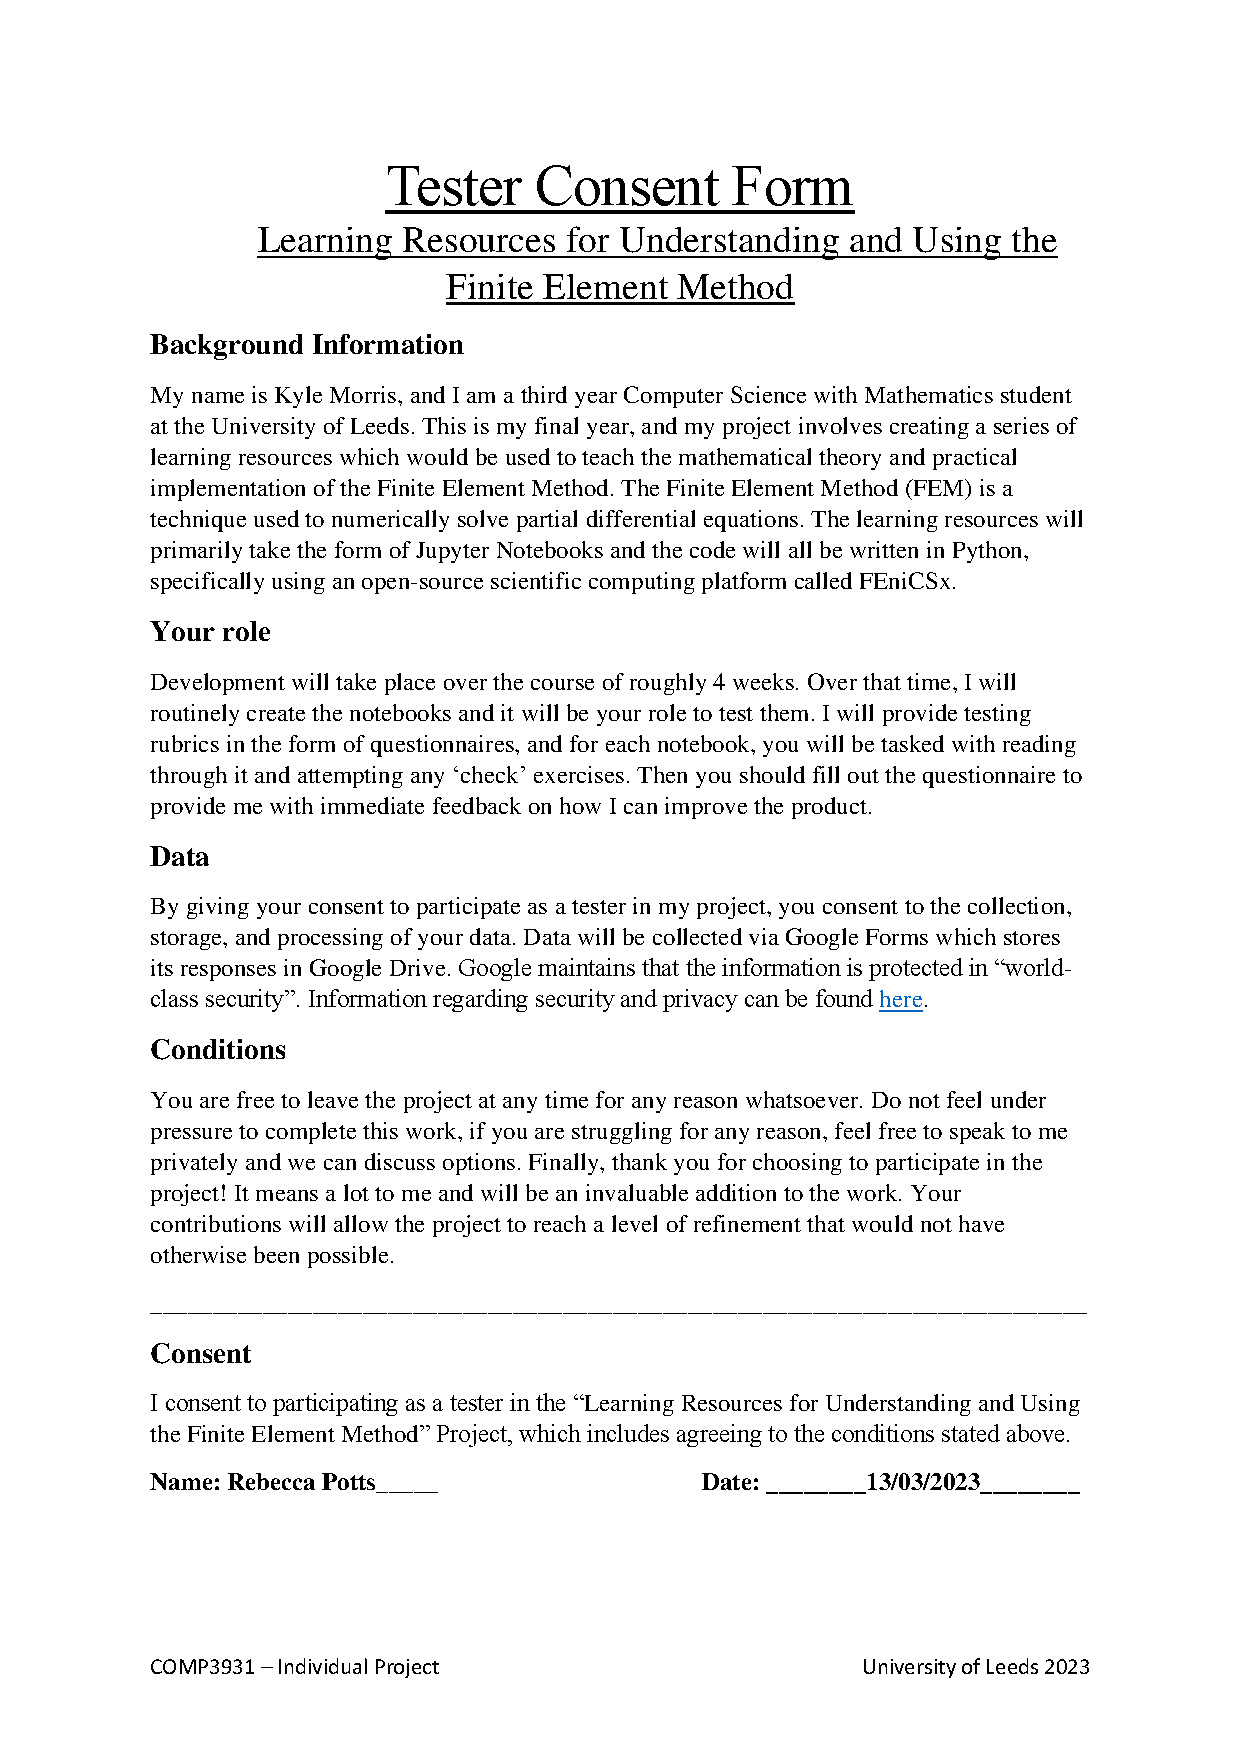
\includepdf{images/consent-forms/beck.pdf}
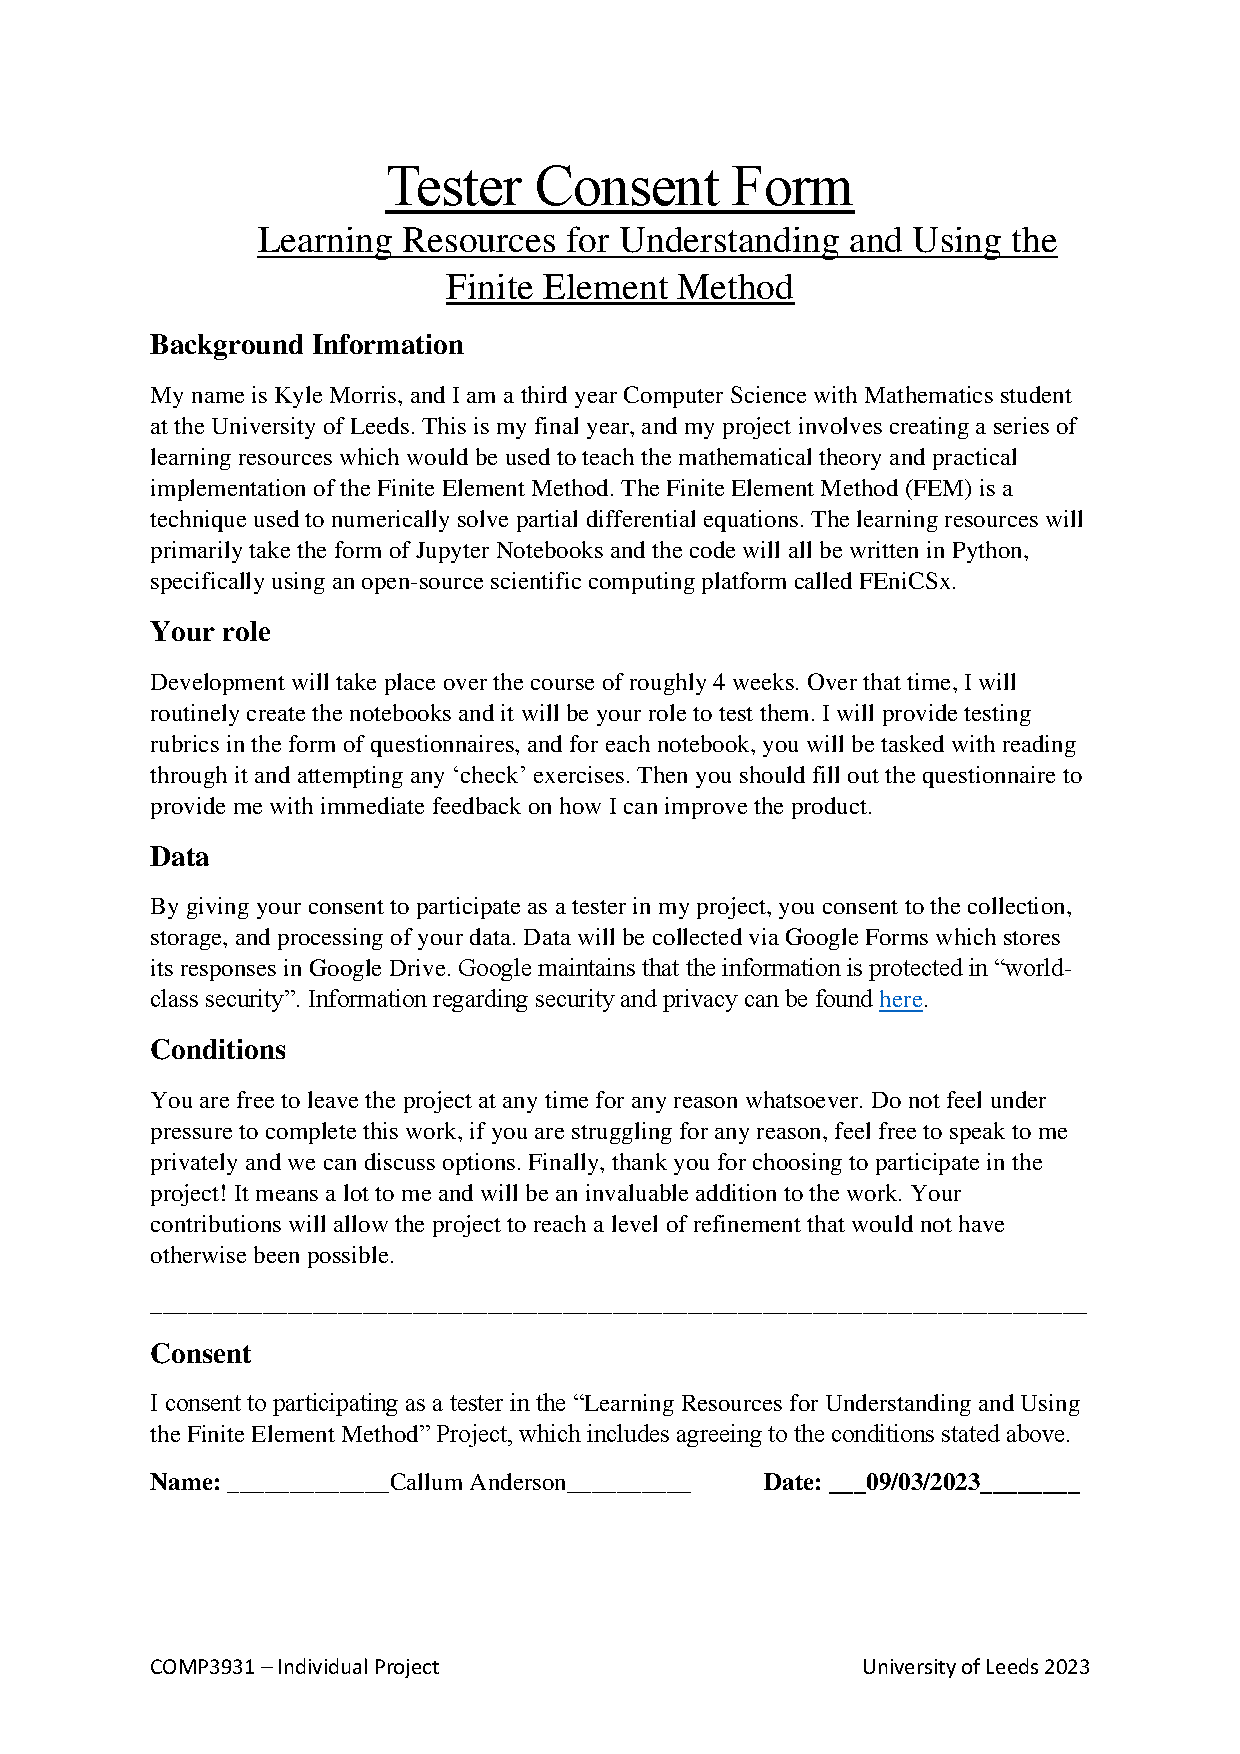
\includepdf{images/consent-forms/callum.pdf}
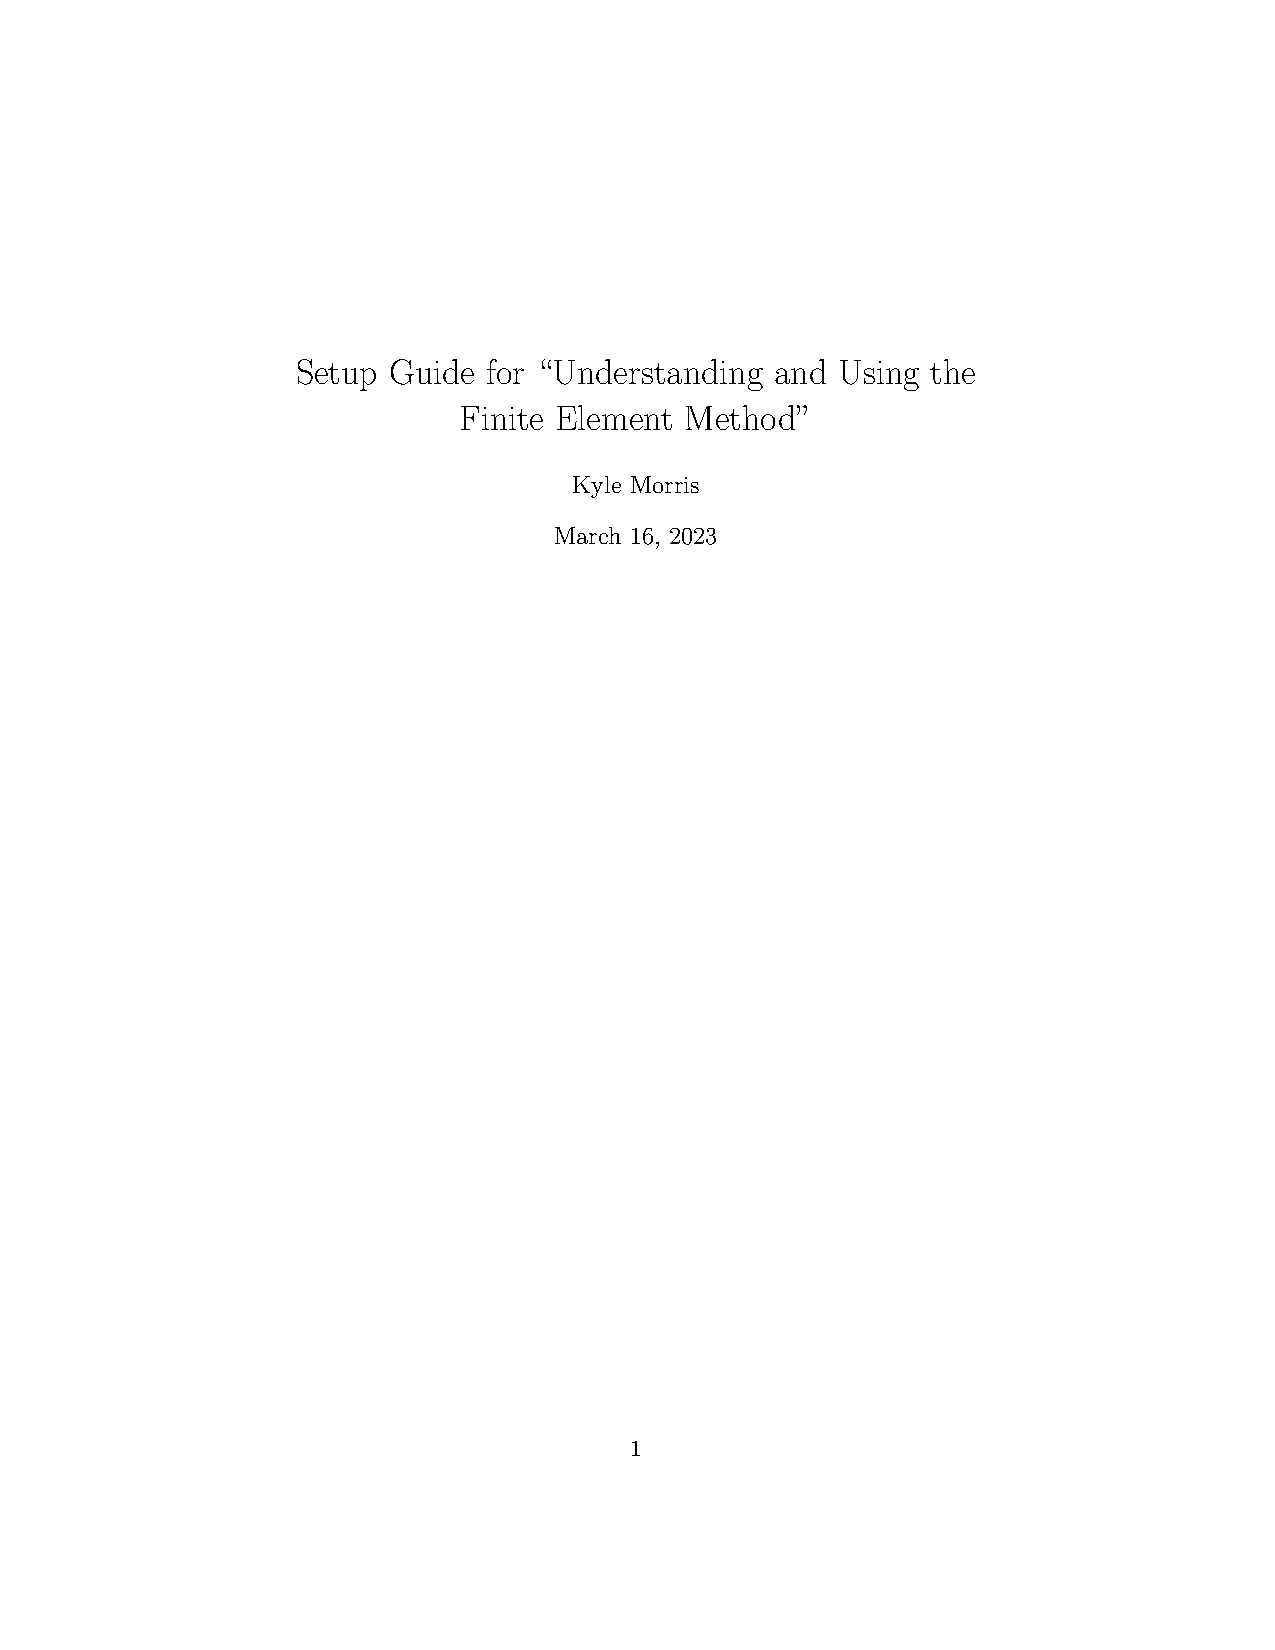
\includepdf[pages=-]{images/misc/setupGuide.pdf}


\end{appendices}
